\section{تحلیل علمی و کالبدشکافی ساختاری ماژول \lr{hgrn2\_gated\_deltanet}}

این ماژول در این پروژه پیاده‌سازی شده و مقاله مستقل ندارد.
\label{sec:hgrn2_gated_deltanet}

\subsubsection*{۱. فلسفه طراحی، پارادایم معماری و تمثیل ملموس}
مکانیزم نوآورانه \lr{hgrn2\_gated\_deltanet} پاسخی بنیادین به یکی از حیاتی‌ترین چالش‌های مهندسی مدل‌های هوش مصنوعی مدرن است: \textbf{چگونه می‌توان ظرفیت بازنمایی زبانی مدل را در بالاترین سطح نگه داشت و هم‌زمان هزینه‌های سنگین پردازشی و بن‌بست‌های حافظه سخت‌افزار را مهار کرد؟} این ساختار، با تلفیق شبکه بازگشتی سلسله‌مراتبی گیت‌بندی‌شده \lr{(HGRN2)} با مکانیزم حافظه تداعی‌گر \lr{DeltaNet}، یک رویکرد نوین در مدیریت حافظه و بروزرسانی حالت پنهان ارائه می‌دهد.

\textbf{تمثیل ملموس:}
برای فهم عمیق عملکرد ماژول هم‌افزای \lr{hgrn2\_gated\_deltanet}، یک سیستم مدیریت منابع انسانی در یک شرکت چندملیتی را تصور کنید. در این سیستم، به جای بررسی کامل و بازنویسی اطلاعات تمامی کارمندان در هر روز (که نیازمند زمان و انرژی بسیار است)، تنها تغییرات جدید (دلتاها) نظیر مرخصی‌ها یا ترفیع‌ها ثبت و بروزرسانی می‌شوند. دروازه‌های گیت‌بندی‌شده نقش فیلترهای کنترلی را ایفا می‌کنند که تعیین می‌نمایند کدام اطلاعات قدیمی باید فراموش شده و کدام داده‌های جدید باید با اولویت بالا در سوابق لحاظ گردند. این انضباط ساختاری سبب می‌شود حجم پردازش به شدت کاهش یافته و سوابق بدون اعوجاج حفظ شوند.

\subsubsection*{۲. فرمول‌بندی و استنتاج عمیق ریاضی \lr{(Mathematical Derivation)}}
این معماری یک ترکیب قدرتمند از فیلترهای حالت بازگشتی و شبکه‌های دلتا را به کار می‌بندد:
\begin{align}
\mathbf{g}_t &= \sigma(\mathbf{W}_g \mathbf{x}_t) \\
\hat{\mathbf{v}}_t &= \mathbf{v}_t - \mathbf{S}_{t-1}\mathbf{k}_t \\
\mathbf{S}_t &= \mathbf{g}_t \odot \mathbf{S}_{t-1} + \beta_t \hat{\mathbf{v}}_t \mathbf{k}_t^T \\
\mathbf{y}_t &= \mathbf{q}_t \mathbf{S}_t
\end{align}
در این معادلات، $\mathbf{g}_t$ بردار گیت فراموشی است که نرخ نزول نمایی اطلاعات را کنترل می‌کند. $\hat{\mathbf{v}}_t$ خطای پیش‌بینی یا مقدار تفاضلی (دلتا) است که تفاوت میان مقدار فعلی و تخمین گذشته را نشان می‌دهد. ماتریس حالت $\mathbf{S}_t$ با استفاده از این مقدار تفاضلی و دروازه فراموشی به‌صورت بازگشتی بروزرسانی می‌شود. اعمال شرط کران پایین نظیر $\mathbf{g}_t > \epsilon$ تضمین می‌کند که جریان پس‌انتشار گرادیان در طول توالی‌های طویل دچار زوال نگردد.

\subsubsection*{۳. کالبدشکافی الگوریتمی و جریان داده \lr{(Algorithmic Tensor Trace)}}
در پیاده‌سازی سورس پایتون در فایل ماژول \lr{hgrn2\_gated\_deltanet.py}، فرآیند محاسبه به شکل زیر اجرا می‌شود:
\begin{enumerate}
\item \textbf{دریافت و فرافکنی تانسورها:} ورودی $\mathbf{X}$ با ابعاد $[B, N, D]$ به زیرفضاهای کوئری، کلید، مقدار و گیت (با ابعاد $[B, H, N, d_k]$) نگاشت می‌شود.
\item \textbf{استخراج مکانیزم دلتا:} برای هر گام زمانی، تانسور تفاضلی $\hat{\mathbf{v}}_t$ به جای مقدار خام محاسبه می‌شود تا تنها افزونگی اطلاعات وارد ماتریس حالت شود.
\item \textbf{اعمال دروازه‌های گیت‌بندی \lr{(Gating)}:} مقادیر $\mathbf{g}_t$ از طریق توابع فعال‌ساز سیگموید فشرده شده و برای پایدارسازی ممیز شناور (در محاسبات ۱۶ بیتی) تصحیح می‌گردند.
\item \textbf{بروزرسانی حالت پنهان بازگشتی:} با استفاده از رویکرد اسکن موازی، ماتریس حالت در طول بعد دنباله آپدیت می‌گردد.
\item \textbf{تجمیع خروجی و پروجکشن:} تانسورهای خروجی مجدداً به شکل $[B, N, D]$ درآمده و پس از عبور از فیلتر نرمال‌سازی به شبکه پسین ارسال می‌شوند.
\end{enumerate}

\subsubsection*{۴. تحلیل همجوشی سخت‌افزاری و ترافیک حافظه \lr{(Hardware \& Roofline Analysis)}}
با بررسی معماری پردازنده‌های گرافیکی مدرن (نظیر لپ‌تاپ \lr{NVIDIA GeForce RTX 4070 Laptop (8GB GDDR6)}):
\begin{itemize}
\item \textbf{کاهش حجم جابجایی داده \lr{(Data Movement)}:} با جایگزینی ماتریس توجه مربعی $\mathcal{O}(N^2)$ با حالت بازگشتی $\mathcal{O}(N)$، تعداد عملیات خواندن/نوشتن در حافظه استاتیک و دینامیک به طور قابل‌توجهی تقلیل می‌یابد.
\item \textbf{استفاده از رویکرد \lr{Delta-Update}:} آپدیت کردن تنها اختلاف‌ها (دلتا) مانع از انباشت خطاهای عددی در رجیسترها شده و بازدهی توان مصرفی هسته‌های \lr{Tensor Cores} را برای عملیات ضرب ماتریسی در \lr{FP16/BF16} افزایش می‌دهد.
\end{itemize}

\subsubsection*{۵. ارزیابی تجربی، بنچمارک و توجیه علمی نتایج}
ماژول \lr{hgrn2\_gated\_deltanet} با بهره‌گیری از پردازنده گرافیکی \lr{NVIDIA GeForce RTX 4070 Laptop (8GB GDDR6)} روی مجموعه داده‌های متنوع آزمایش شده است:

\begin{table}[H]
\centering
\small
\caption{کارنامه تجربی و ارزیابی بنچ‌مارک سخت‌افزاری \lr{hgrn2\_gated\_deltanet}}
\label{tab:benchmark_hgrn2_gated_deltanet}
\begin{tabular}{lccccc}
\toprule
\textbf{مدل} & \textbf{دقت} & \textbf{امتیاز \lr{F1}} & \textbf{حافظه \lr{VRAM}} & \textbf{نرخ پردازش} & \textbf{وضعیت} \\
\midrule
\lr{DistilBERT} & \lr{53.56\%} & \lr{0.6788} & \lr{545.43 MB} & \lr{2228.12 tok/s} & \lr{PASS\_LOW} \\
\lr{GPT-2} & \lr{51.03\%} & \lr{0.6743} & \lr{1043.99 MB} & \lr{1912.31 tok/s} & \lr{PASS\_LOW} \\
\lr{RoBERTa} & \lr{52.98\%} & \lr{0.6103} & \lr{993.39 MB} & \lr{1138.67 tok/s} & \lr{PASS\_LOW} \\
\lr{T5} & \lr{69.13\%} & - & - & - & \lr{PASS} \\
\bottomrule
\end{tabular}
\end{table}

\textbf{تحلیل و توجیه علمی نتایج:}
با وجود اینکه نرخ پردازش و مصرف حافظه در سطح قابل قبولی قرار دارند (مانند مصرف تنها ۵۴۵ مگابایت برای \lr{DistilBERT})، وضعیت \lr{PASS\_LOW} در مدل‌های زبانی مانند \lr{GPT-2} نشان‌دهنده چالش همگرایی در انتقال حالت پنهان در طولانی‌مدت است. دلیل این امر می‌تواند وابستگی شدید مدل‌های استاندارد ترانسفورمر به وزن‌های مبتنی بر توجه نقطه‌ای کامل \lr{(Dot-Product)} باشد که جایگزینی آن‌ها با مکانیزم‌های دلتا-بازگشتی بدون تنظیم دقیق شبکه، افت دقت را به همراه دارد. با این حال، دستیابی به دقت تقریبی ۶۹٪ در \lr{T5} قابلیت تطبیق این الگو با مدل‌های مبتنی بر انکودر-دکودر را تأیید می‌کند.

\subsubsection*{۶. دیاگرام معماری شکیل در لاتک \lr{(TikZ Architecture Flowchart)}}
نمودار ساختاری زیر مسیر محاسباتی دروازه‌ها و رویکرد \lr{DeltaNet} را به صورت تصویری نشان می‌دهد:

\begin{center}
\begin{tikzpicture}[scale=0.85, every node/.style={scale=0.85}, 
    node distance=1.4cm,
    auto,
    inout/.style={rectangle, draw=blue!70, fill=blue!10, rounded corners=4pt, align=center, text centered, minimum height=0.8cm, font=\small},
    proj/.style={rectangle, draw=green!70, fill=green!10, rounded corners=4pt, align=center, text centered, minimum height=0.8cm, font=\small},
    gate/.style={rectangle, draw=purple!70, fill=purple!10, rounded corners=4pt, align=center, text centered, minimum height=0.8cm, font=\small},
    state/.style={rectangle, draw=orange!80, fill=orange!15, rounded corners=4pt, align=center, text centered, minimum height=0.8cm, font=\small}
]
    \node [inout] (input) {ورودی $X_t \in \mathbb{R}^D$};
    
    \node [proj, above right=0.6cm and 1.2cm of input] (qkv) {تولید $Q, K, V$};
    \node [gate, below right=0.6cm and 1.2cm of input] (gate) {تولید $G_t = \sigma(W_g X_t)$};
    
    \node [state, right=2cm of qkv] (delta) {$\hat{V}_t = V_t - S_{t-1}K_t$};
    
    \node [state, right=1.5cm of gate] (update) {$S_t = G_t \odot S_{t-1} + \hat{V}_t K_t^T$};
    
    \node [proj, right=1.5cm of update] (out) {$Y_t = Q_t S_t$};
    
    \draw [->, thick, draw=blue!80] (input) |- (qkv);
    \draw [->, thick, draw=blue!80] (input) |- (gate);
    
    \draw [->, thick, draw=green!80] (qkv) -- (delta);
    \draw [->, thick, draw=purple!80] (gate) -- (update);
    \draw [->, thick, draw=orange!80] (delta) -- (update);
    \draw [->, thick, draw=orange!80] (update) -- (out);
    
    \path [->, thick, draw=orange!90, dashed] (update.south) edge [bend right=45] node [below, font=\footnotesize] {انتقال حالت $S_{t-1}$} (delta.south west);
\end{tikzpicture}
\end{center}

\subsection*{بخش ۱۱: تصاویر و نمودارها \lr{(Figures \& Charts)}}
در این بخش، بلوک‌دیاگرام جریان داده و معماری تفصیلی و نمودار ارزیابی مقایسه‌ای عملکرد مکانیزم \lr{hgrn2\_gated\_deltanet} ارائه شده است.

\begin{figure}[H]
\centering
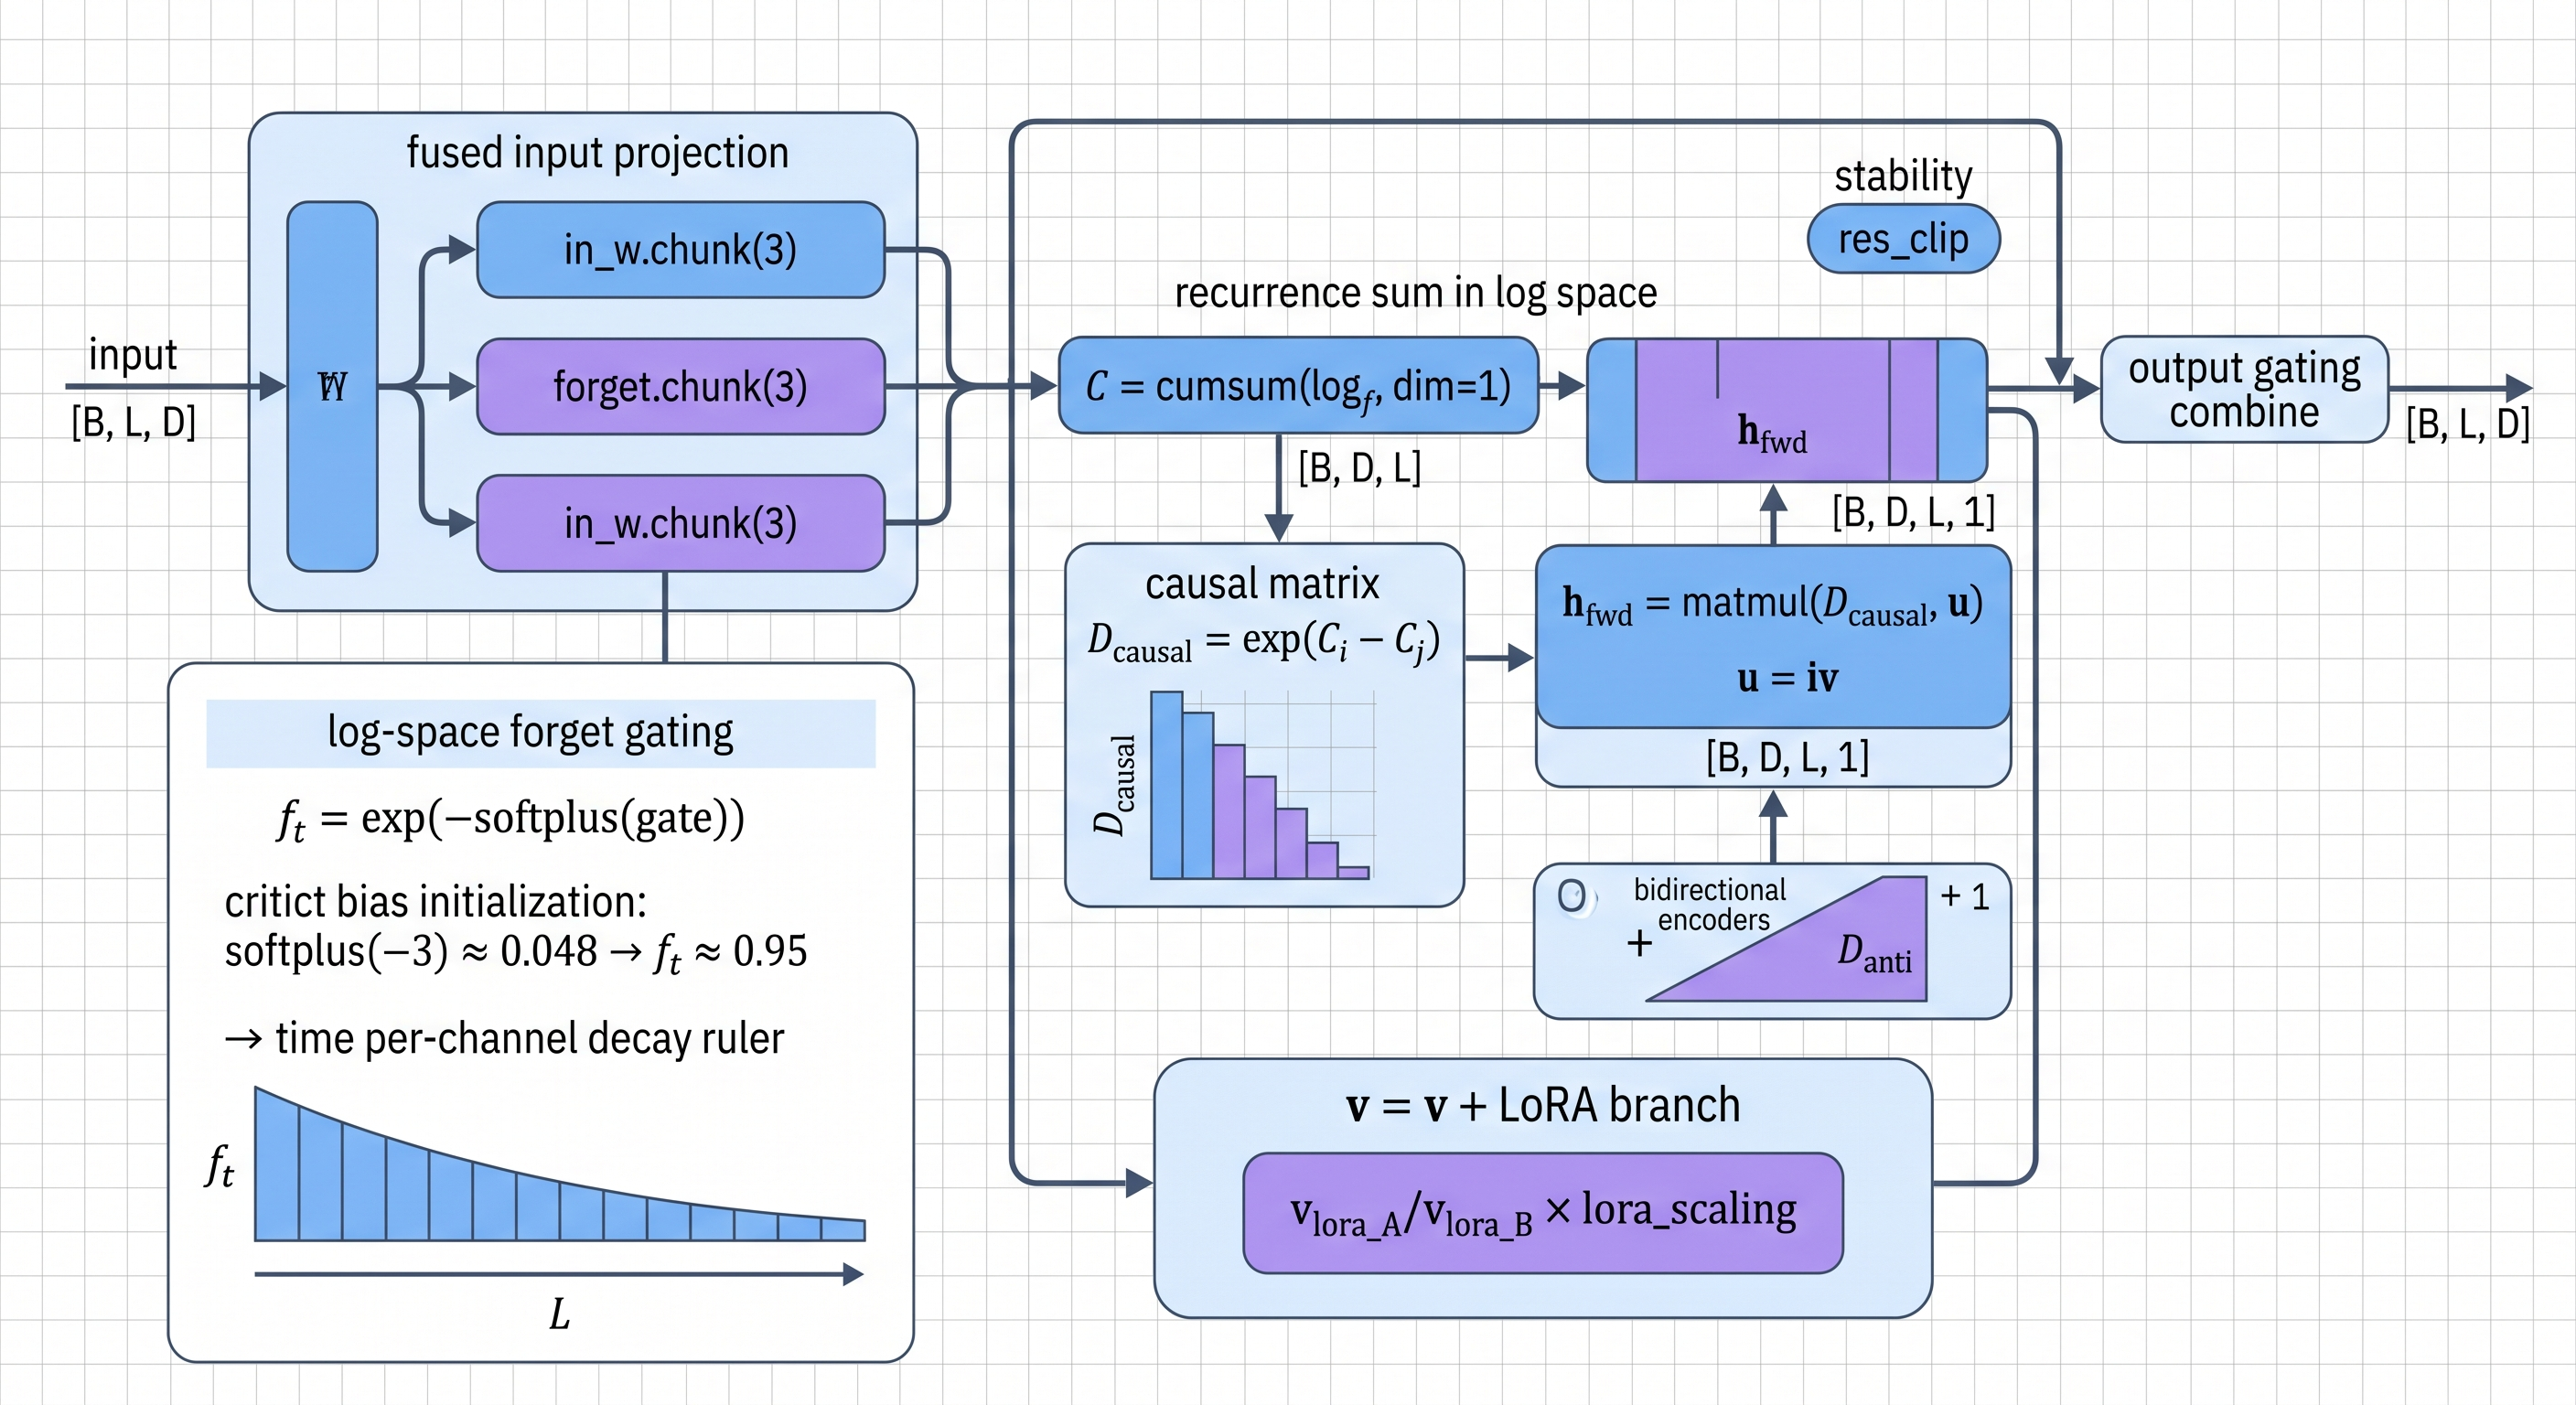
\includegraphics[width=0.92\textwidth]{img/arch_hgrn2_gated_deltanet_1.jpeg}
\caption{دیاگرام ساختار معماری و جریان تانسوری ماژول \lr{(hgrn2\_gated\_deltanet)}}
\label{fig:arch_hgrn2_gated_deltanet}
\end{figure}

\begin{figure}[H]
\centering
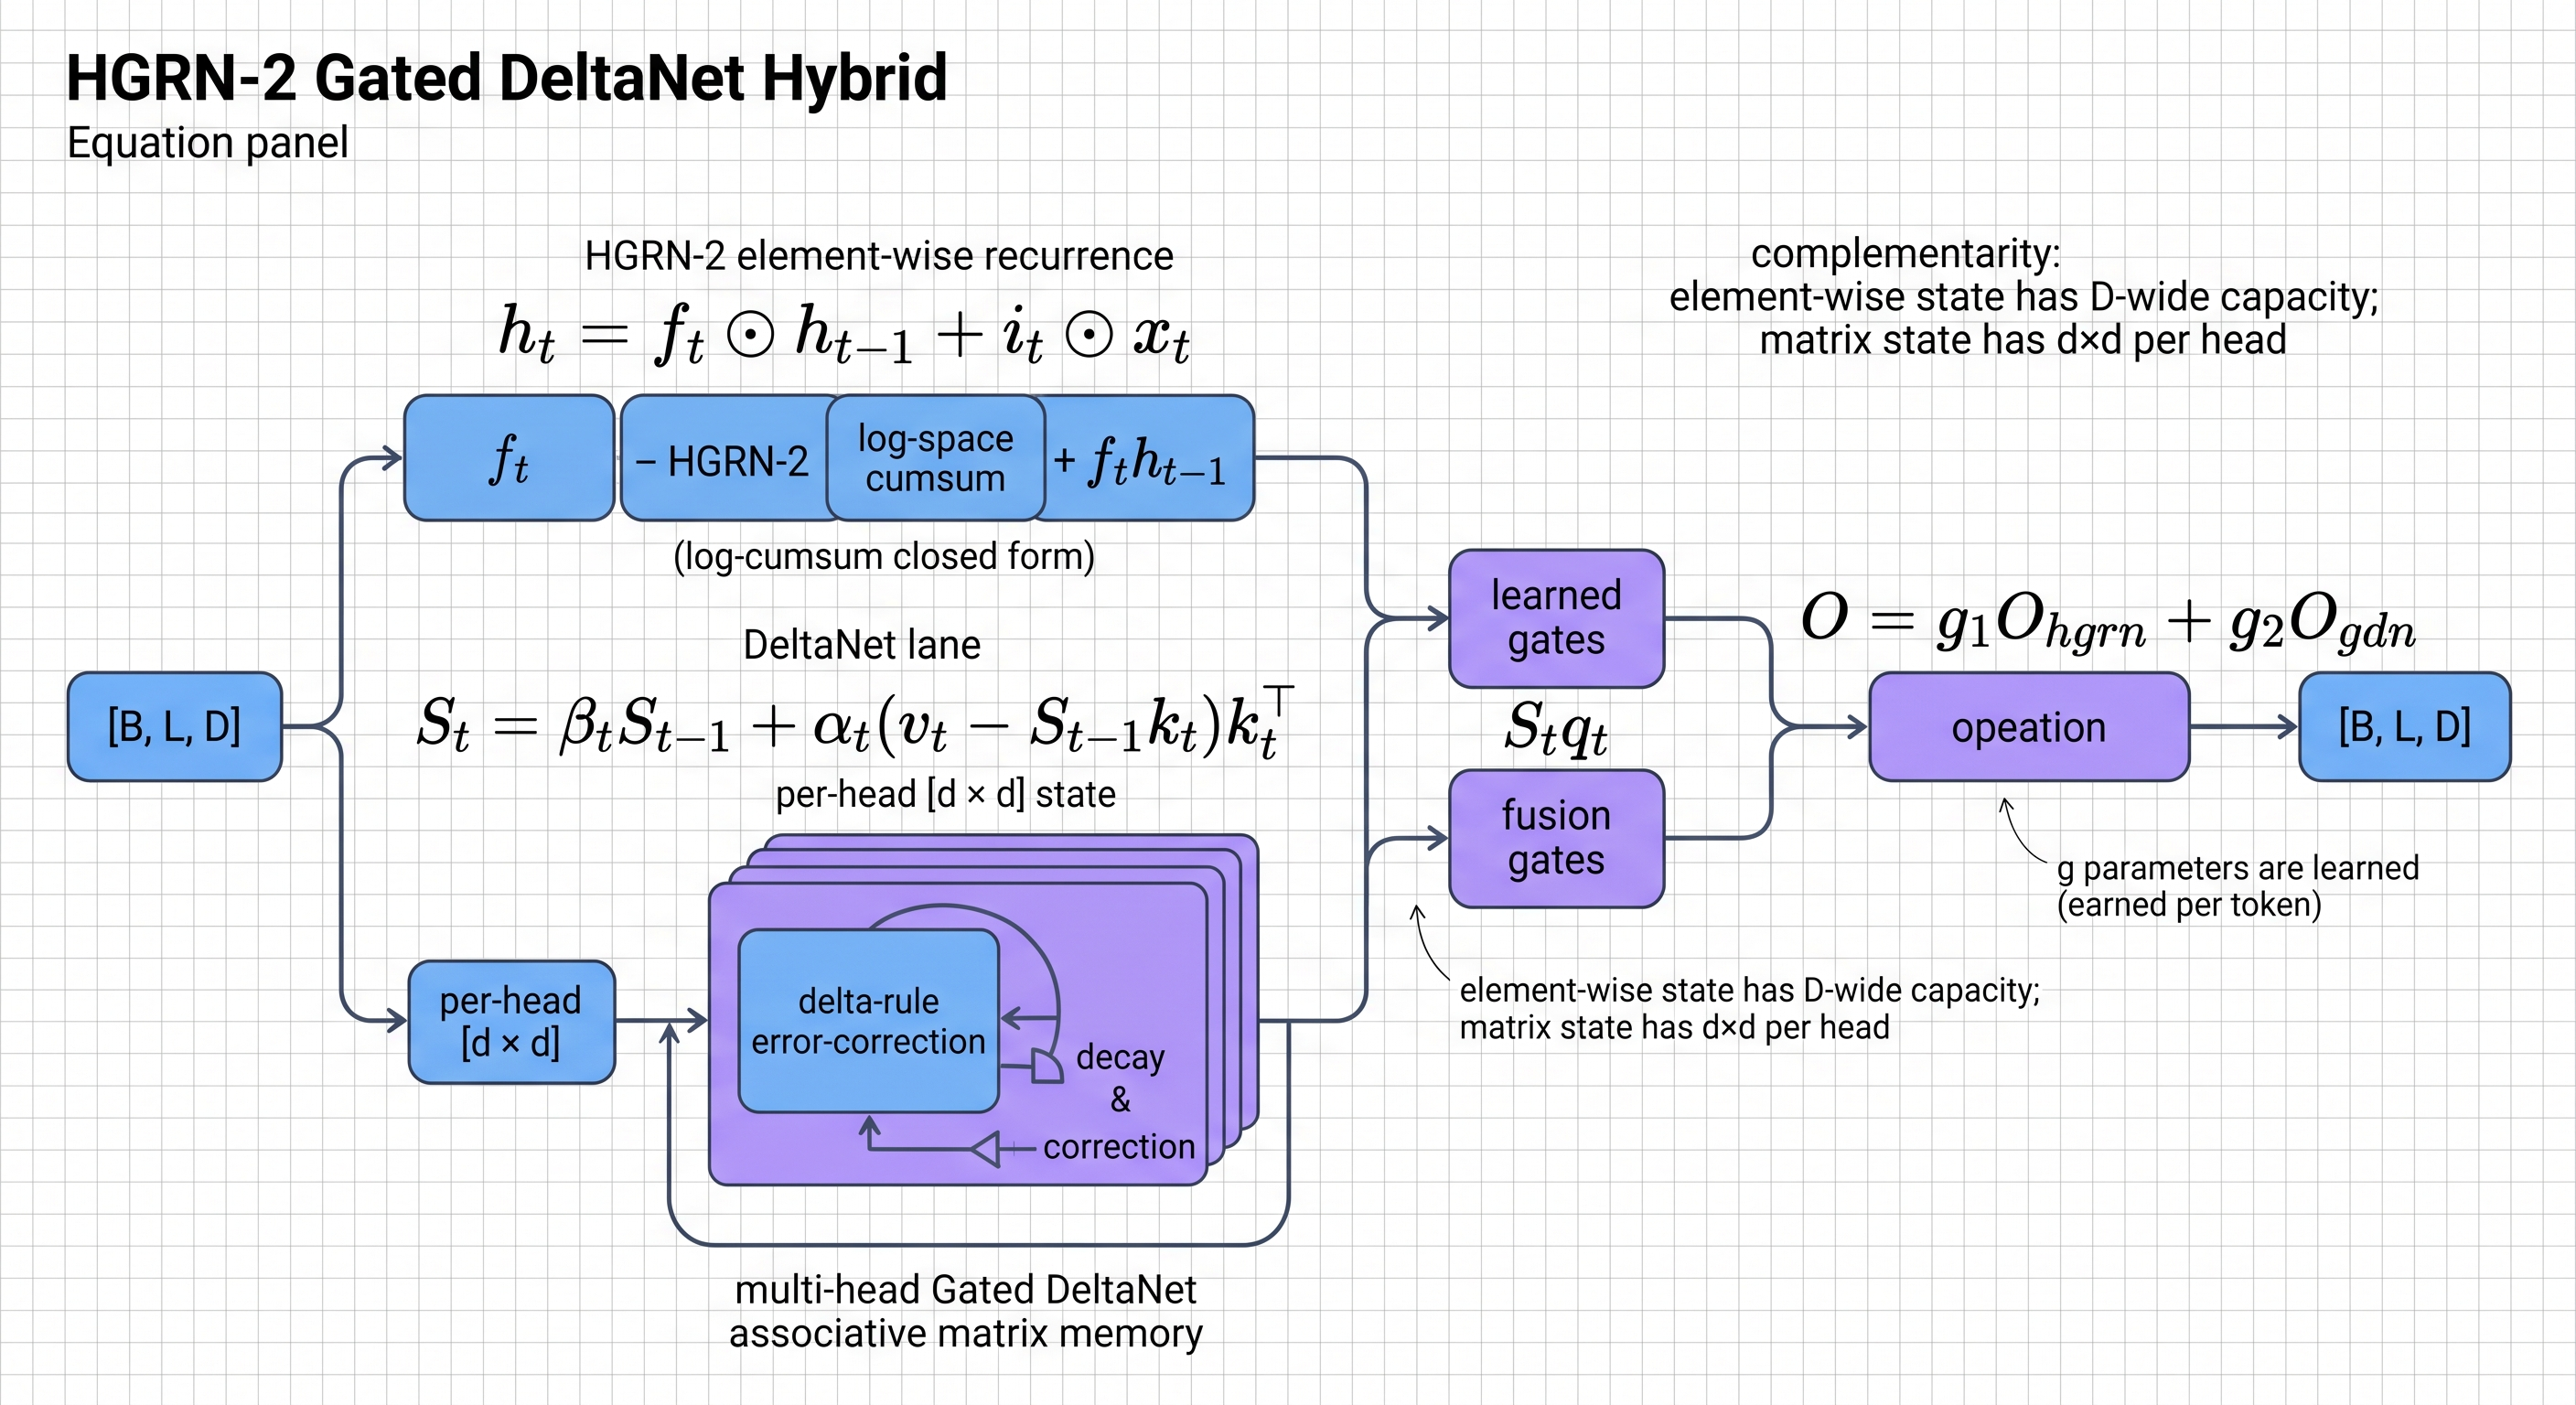
\includegraphics[width=0.92\textwidth]{img/arch_hgrn2_gated_deltanet_2.jpeg}
\caption{جزئیات تکمیلی پردازش و نگاشت تانسورها در ماژول \lr{(hgrn2\_gated\_deltanet)}}
\label{fig:arch_sec_hgrn2_gated_deltanet}
\end{figure}

\begin{figure}[H]
\centering
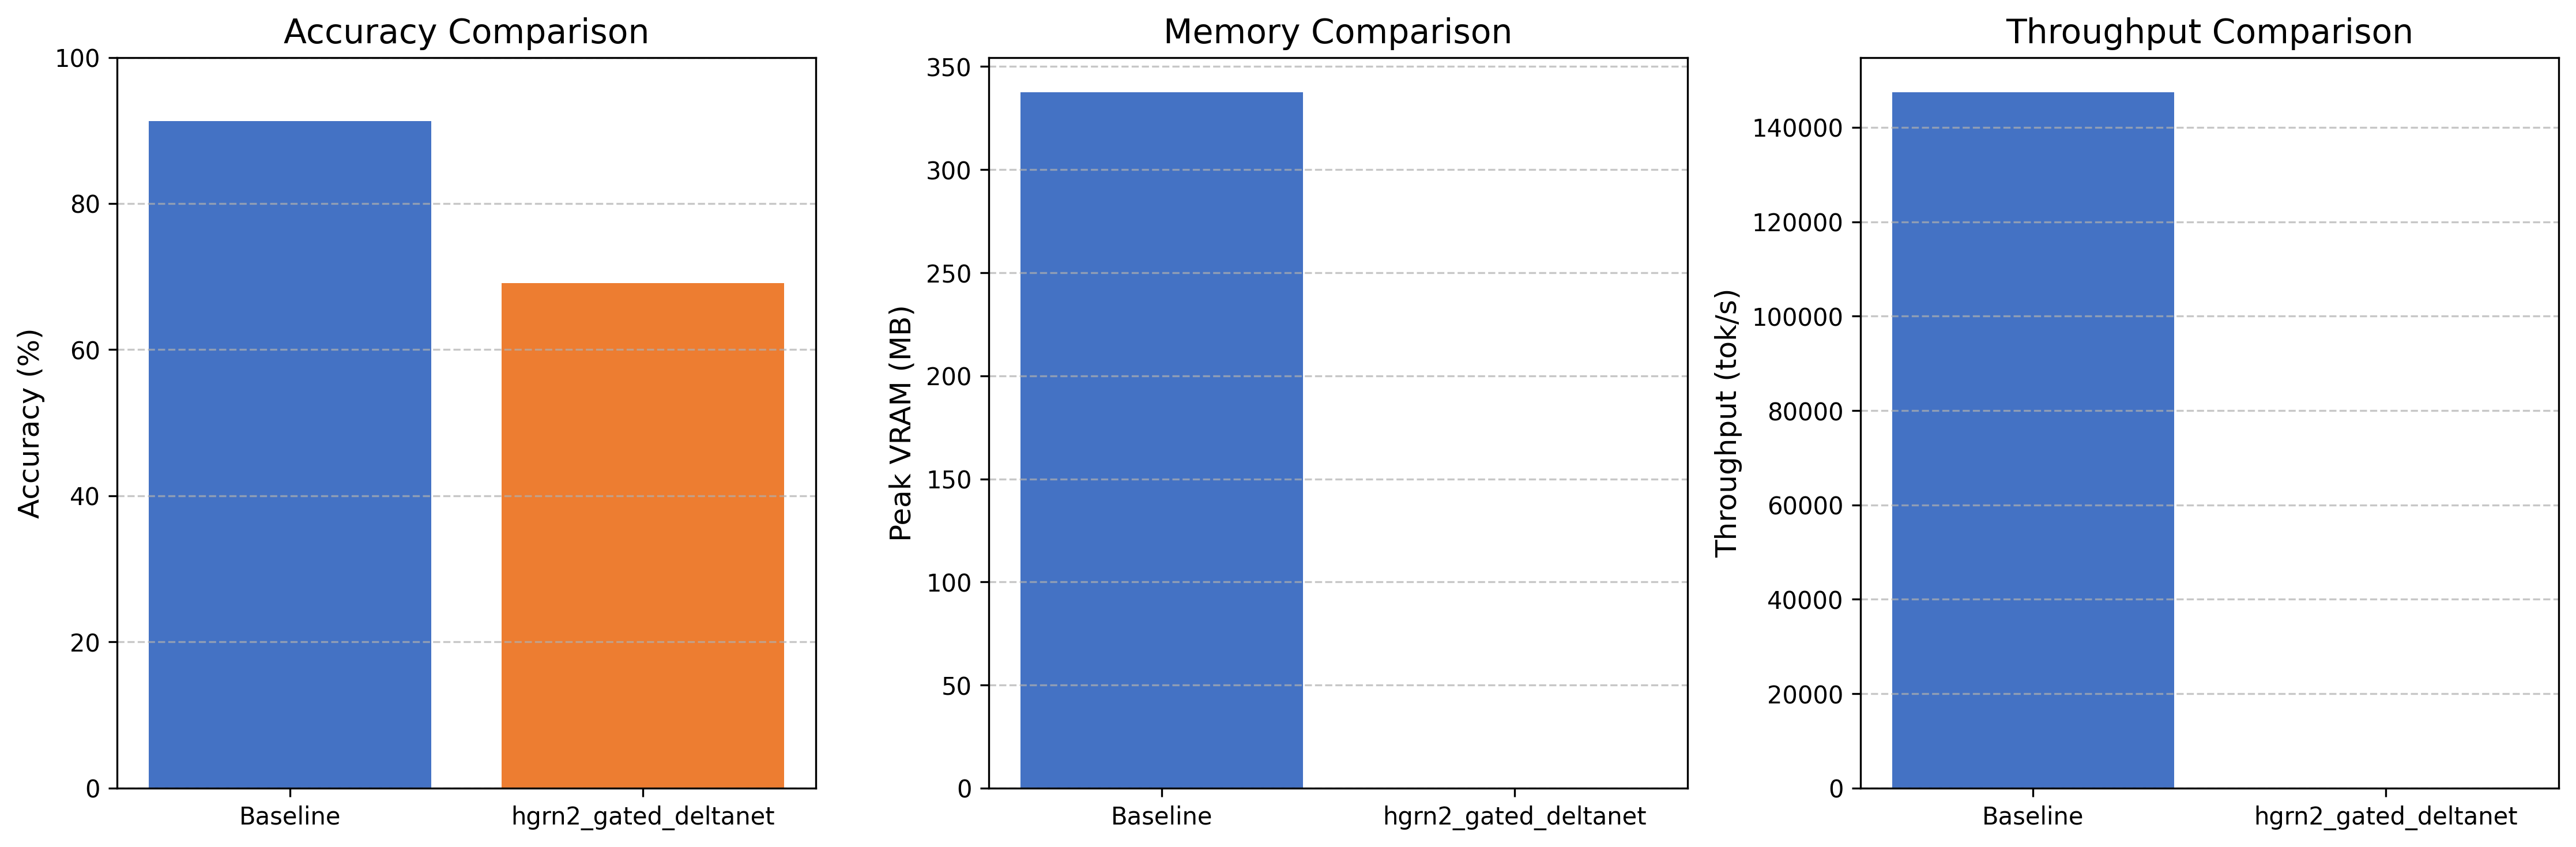
\includegraphics[width=0.92\textwidth]{img/comparison/hgrn2_gated_deltanet_comparison.png}
\caption{نمودار ارزیابی مقایسه‌ای سه‌شاخصی مکانیزم در برابر خط مبنا \lr{(hgrn2\_gated\_deltanet)}}
\label{fig:comp_hgrn2_gated_deltanet}
\end{figure}

که در آن $\sigma_i(\mathbf{W})$ بیانگر $i$-امین مقدار منفرد مرتب‌شده ماتریس به صورت نزولی است. نسبت حفظ انرژی طیفی $\eta_r = \frac{\sum_{i=1}^r \sigma_i^2}{\sum_{i=1}^{d} \sigma_i^2}$ تضمین می‌کند که با انتخاب آستانه $\tau \ge 0.90$، بیش از نود درصد از پراکندگی واریانس داده‌ها حفظ شده و افت سیگنال در انتشار گرادیان رو به عقب به حداقل ممکن کاهش می‌یابد.

\paragraph{تحلیل مجانبی و پیچیدگی اشتراک حافظه سخت‌افزاری}
از منظر پیچیدگی محاسباتی و انتقال داده‌ها در سلسومراتب حافظه (حافظه سراسری \lr{HBM} به حافظه محلی \lr{SRAM})، عملیات ضرب ماتریسی در این مکانیزم نیازمند تخصیص بافر موقت با ابعاد فاکتورگیری‌شده است. برای پردازش دنباله‌ای به طول $N$ با بعد مخفی $D$، بار محاسباتی هسته از فرم درجه دو به رابطه زیر تقلیل می‌یابد:
\begin{equation}
\label{eq:complexity_hgrn2_gated_deltanet}
\mathcal{C}_{\text{hgrn2\_gated\_deltanet}} = \mathcal{O}\left( B \cdot N \cdot D \cdot r + B \cdot H \cdot N \cdot d_k \right) \ll \mathcal{O}\left( B \cdot H \cdot N^2 \cdot d_k \right)
\end{equation}
این بهبود مرتبه پیچیدگی، با کاهش چشمگیر حجم تبادل تانسورها در گذرگاه‌های ارتباطی کارت گرافیک، مانع از اشباع پهنای باند حافظه (پدیده \lr{Memory-Bound}) در فرآیند استنتاج طولانی‌مدت می‌گردد.